\documentclass[a4paper,10pt]{article}
\usepackage[utf8]{inputenc}
\usepackage[english]{babel}
\usepackage{geometry}
\usepackage{graphicx}
\usepackage{blindtext}
\usepackage{titling}
\usepackage[nottoc]{tocbibind} %Adds "References" to the table of contents
\usepackage{fontawesome}
\usepackage{url}
\usepackage{hyperref}
\usepackage{float}
\usepackage{subcaption}
\usepackage{color}
\hypersetup{
	colorlinks=true,
	linkcolor=black,
	filecolor=magenta,      
	urlcolor=blue,
}


\newcommand{\github}[2][13pt]{\hspace{5pt}\faGithub\hspace{5pt}\fontsize{#1}{0}\url{#2}}

%Document title, author and date (empty)
\title{Game of Life}
\author{Giovanni Sorice - 606915}
\date{April 2020}

% Definition of \maketitle
\makeatletter         
\def\@maketitle{
	\raggedright
	%\includegraphics[width = 40mm]{logo.jpg}\\[8ex]
	\begin{center}
		{\Huge \bfseries \sffamily \@title }\\[4ex] 
		{\Large  \@author}\\[4ex] 
		\@date\\[8ex]
		
\includegraphics[scale = 0.35]{logo-Pisa.jpeg}
\end{center}}
\makeatother

%Beginning of the document
\begin{document}
	

		\maketitle
		\begin{abstract}
			The assignment required to implement different solutions for Conway's Game of Life. I initially developed a \textit{sequential} version, needed as a baseline and performance comparison for further implementations. The parallel versions developed are several.
		\end{abstract}

	
	
	\section{Measures}
	We need some measures to understand the real advantages of using a parallel implementation. The common measures used in this case are speedup and scalability.
	\subsection{Speedup}
	The speedup is used to compare the time needed to execute a specific task sequentially with the time needed to do the same task in parallel. The ratio among the time spent by the sequential and the time spent by the parallel is called Speedup. We hope that it was linearly proportional to the number of parallel degree used and for this reason the time spent doing the task decrease as 1/k where k is the parallelism degree. Unfortunately, there are more things to keep in mind (overhead) and usually the rate of speedup is not the expected.
	The speedup is computed as follows.
	\begin{equation}
	speedup(n)=\frac{T_{seq}}{T_{par}}
	\end{equation}
	
	\subsection{Scalability}
	The scalability is the ration between the parallel execution time with parallelism degree equal to 1 and the parallel execution time with parallelism degree equal to n.
		\begin{equation}
	scalab(n)=\frac{T_{par}(1)}{T_{par}(n)}
	\end{equation}
	\section{Implementation structure}
	I defined four classes:\textit{GoLSeq}, \textit{GoLThread},\textit{GoLOMP} and \textit{GoLPool} in which there are respectively the implementation of the sequential code, parallel code with c++ standard thread used as fork-join, parallel code with OpenMP and parallel code with c++ standard thread used as a pool of worker and queue of tasks.
	The results of pool version are  really good when I use small matrices but very bad in big matrices. I think that this behavior is influenced by the bottleneck in the queue of tasks in which the matrix is decomposed cell by cell.   
	For this reason, the graph with big amount of rows and columns are not displayed with the pool implementation.
	All the code could be found at \url{https://github.com/GiovanniSorice/GameOfLife}.

	\section{Results}
	The results are shown in graphs, all the execution are made on square matrices. The size tested are 500x500, 1000x1000, 5000x5000 and 1000x1000 with 15 iterations.
	The test are made on Xeon Phi. 
	
	\subsection{Speedup graph}
	\begin{figure}[H]
		\centering
		\begin{minipage}[t]{0.55\linewidth}
			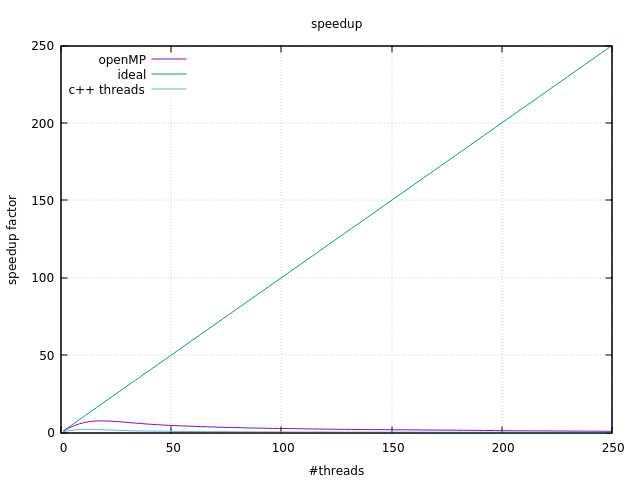
\includegraphics[width=\linewidth]{BenchMarkGOL/speedup/500/graph500.png}
			%\subcaption{MSE}
		\end{minipage}%
		\begin{minipage}[t]{0.55\linewidth}
			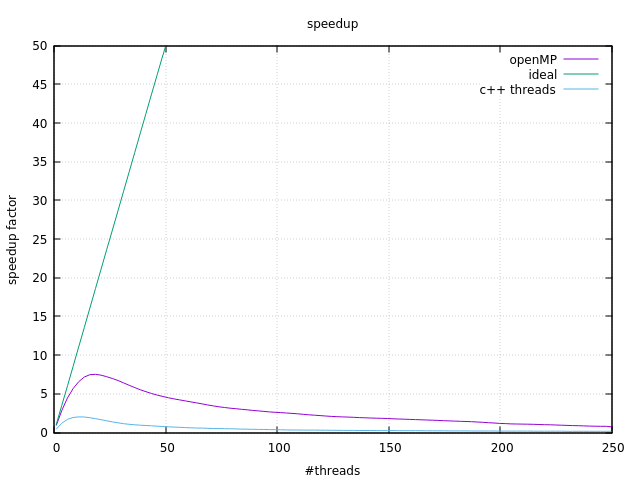
\includegraphics[width=\linewidth]{BenchMarkGOL/speedup/500/graph500_zoom.png}
			%\subcaption{Accuracy}
		\end{minipage}
		\caption{Speedup curves for 500x500 boards.}
		\label{500}
	\end{figure}

	\begin{figure}[H]
		\centering
		\begin{minipage}[t]{0.55\linewidth}
			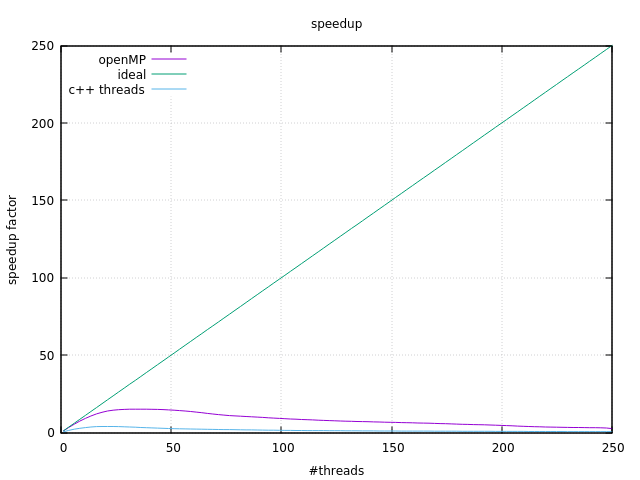
\includegraphics[width=\linewidth]{BenchMarkGOL/speedup/1000/graph1000.png}
			%\subcaption{MSE}
		\end{minipage}%
		\begin{minipage}[t]{0.55\linewidth}
			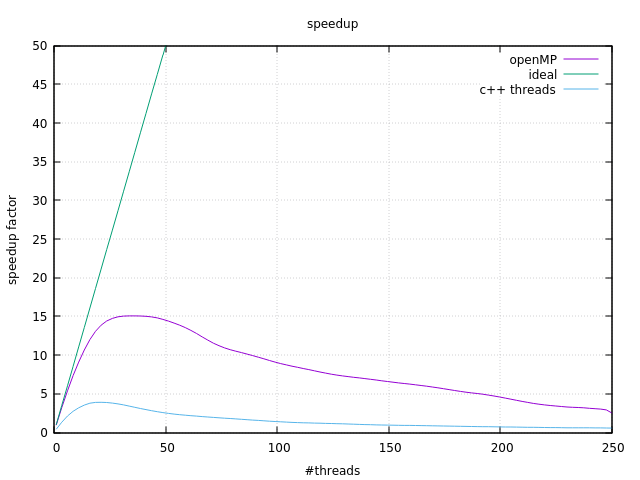
\includegraphics[width=\linewidth]{BenchMarkGOL/speedup/1000/graph1000_zoom.png}
			%\subcaption{Accuracy}
		\end{minipage}
		\caption{Speedup curves for 1000x1000 boards.}
		\label{1000}
	\end{figure}

		\begin{figure}[H]
		\centering
		\begin{minipage}[t]{0.55\linewidth}
			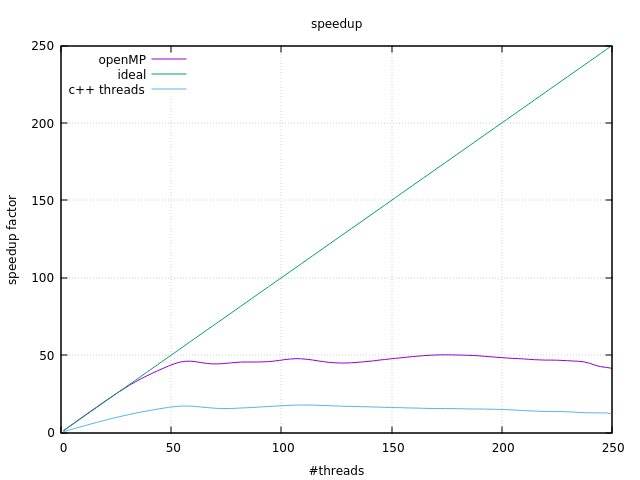
\includegraphics[width=\linewidth]{BenchMarkGOL/speedup/5000/graph5000.png}
			%\subcaption{MSE}
		\end{minipage}%
		\begin{minipage}[t]{0.55\linewidth}
			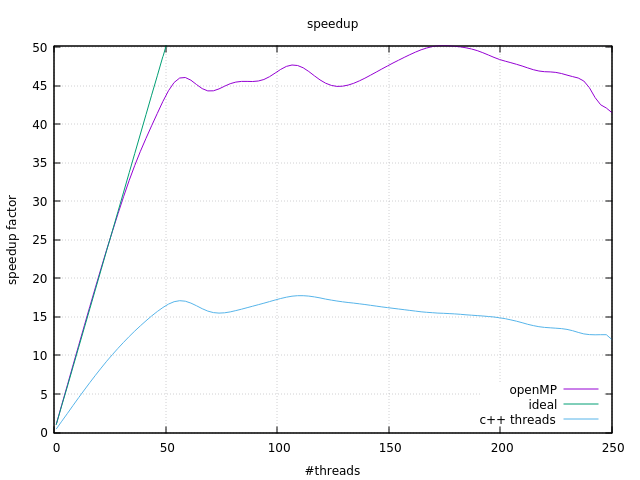
\includegraphics[width=\linewidth]{BenchMarkGOL/speedup/5000/graph5000_zoom.png}
			%\subcaption{Accuracy}
		\end{minipage}
		\caption{Speedup curves for 5000x5000 boards.}
		\label{5000}
	\end{figure}

		\begin{figure}[H]
		\centering
		\begin{minipage}[t]{0.55\linewidth}
			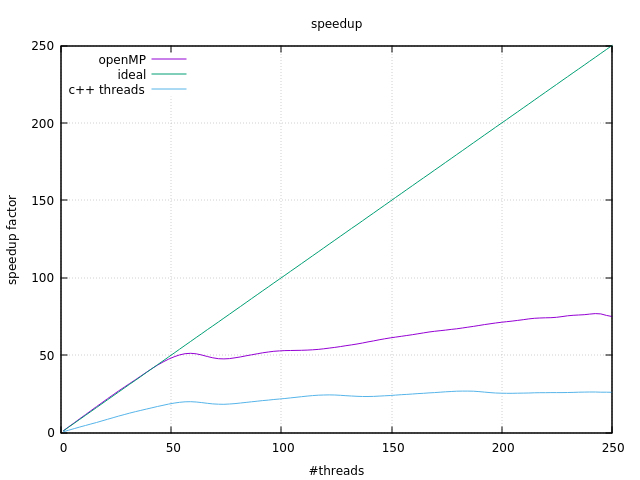
\includegraphics[width=\linewidth]{BenchMarkGOL/speedup/10000/graph10000.png}
			%\subcaption{MSE}
		\end{minipage}%
		\begin{minipage}[t]{0.55\linewidth}
			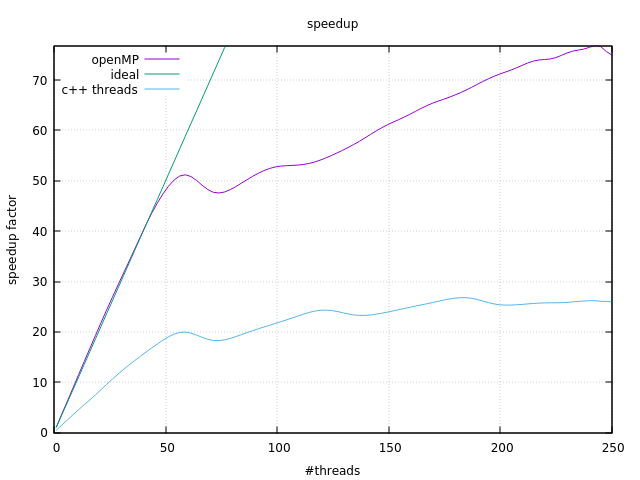
\includegraphics[width=\linewidth]{BenchMarkGOL/speedup/10000/graph10000_zoom.png}
			%\subcaption{Accuracy}
		\end{minipage}
		\caption{Speedup curves for 10000x10000 boards.}
		\label{10000}
	\end{figure}

	\subsection{Scalability graph}
		\begin{figure}[H]
		\centering
		\begin{minipage}[t]{0.55\linewidth}
			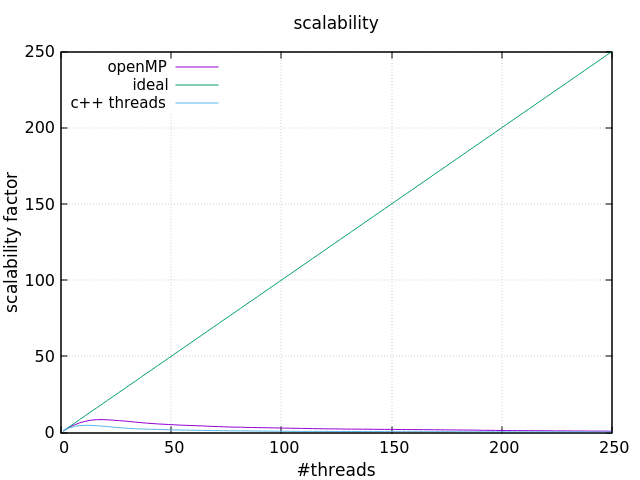
\includegraphics[width=\linewidth]{BenchMarkGOL/scalability/500/graph500_scal.png}
			%\subcaption{MSE}
		\end{minipage}%
		\begin{minipage}[t]{0.55\linewidth}
			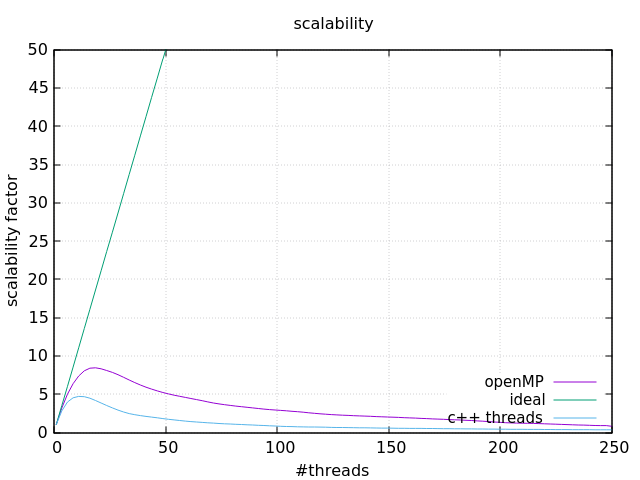
\includegraphics[width=\linewidth]{BenchMarkGOL/scalability/500/graph500_scal_zoom.png}
			%\subcaption{Accuracy}
		\end{minipage}
		\caption{Scalability curves for 500x500 boards.}
		\label{500s}
	\end{figure}

	\begin{figure}[H]
		\centering
		\begin{minipage}[t]{0.55\linewidth}
			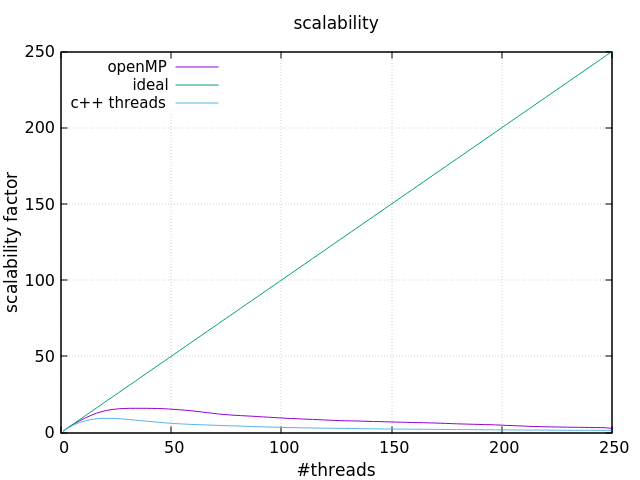
\includegraphics[width=\linewidth]{BenchMarkGOL/scalability/1000/graph1000_scal.png}
			%\subcaption{MSE}
		\end{minipage}%
		\begin{minipage}[t]{0.55\linewidth}
			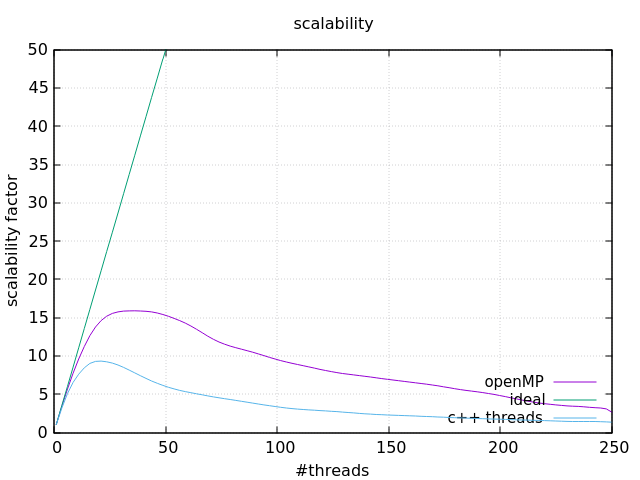
\includegraphics[width=\linewidth]{BenchMarkGOL/scalability/1000/graph1000_scal_zoom.png}
			%\subcaption{Accuracy}
		\end{minipage}
		\caption{Scalability curves for 1000x1000 boards.}
		\label{1000s}
	\end{figure}

	\begin{figure}[H]
		\centering
		\begin{minipage}[t]{0.55\linewidth}
			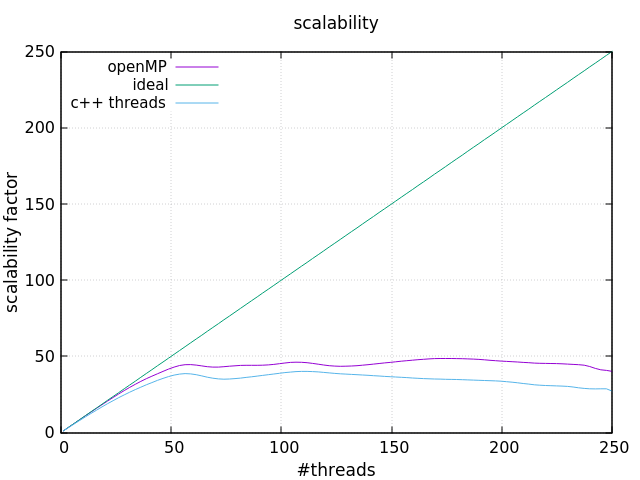
\includegraphics[width=\linewidth]{BenchMarkGOL/scalability/5000/graph5000_scal.png}
			%\subcaption{MSE}
		\end{minipage}%
		\begin{minipage}[t]{0.55\linewidth}
			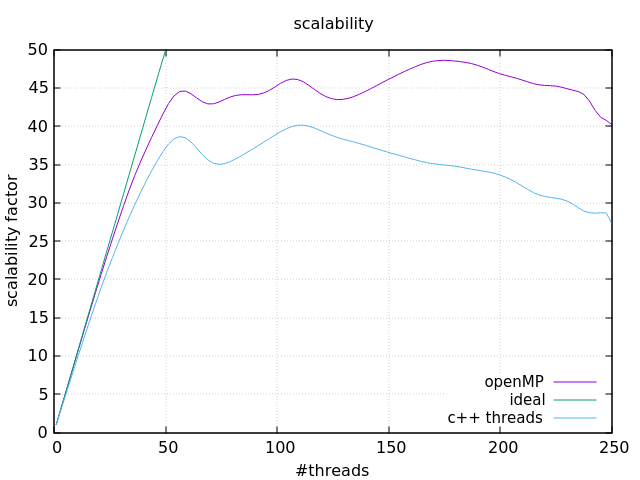
\includegraphics[width=\linewidth]{BenchMarkGOL/scalability/5000/graph5000_scal_zoom.png}
			%\subcaption{Accuracy}
		\end{minipage}
		\caption{Scalability curves for 5000x5000 boards.}
		\label{5000s}
	\end{figure}

	\begin{figure}[H]
		\centering
		\begin{minipage}[t]{0.55\linewidth}
			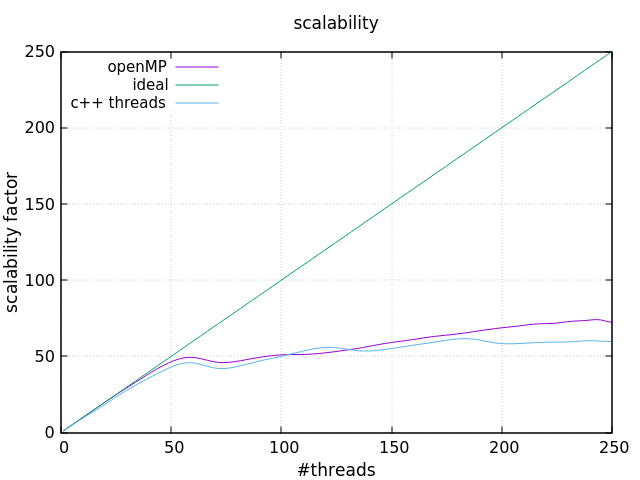
\includegraphics[width=\linewidth]{BenchMarkGOL/scalability/10000/graph10000_scal.png}
			%\subcaption{MSE}
		\end{minipage}%
		\begin{minipage}[t]{0.55\linewidth}
			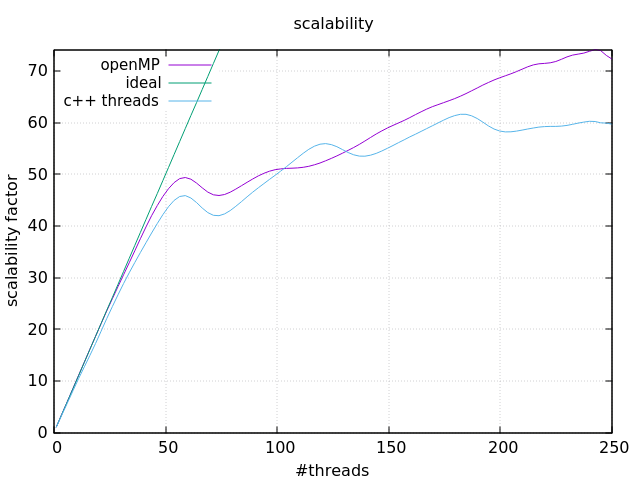
\includegraphics[width=\linewidth]{BenchMarkGOL/scalability/10000/graph10000_scal_zoom.png}
			%\subcaption{Accuracy}
		\end{minipage}
		\caption{Scalability curves for 10000x10000 boards.}
		\label{10000s}
	\end{figure}
\section{Conclusions}
We can see in the graphs that as expected the speedup and the scalability do not increase linearly, but at a certain point reach an inflection point and start decrease or stabilize itself. This can be attribute to the increasing of the overhead of the splitting. In conclusion, it is important to find the right number of parallelism degree and not underestimate the overhead.
\end{document}